\title{Experimental Laboratory 1 - Fluids Labs}
\author{
        Sergio M. Vanegas A.\\
                Department of Mathematics\\
        Polimi---Politecnico di Milano\\
        Milano, Italia
}
\date{\today}

\documentclass[12pt]{article}

\usepackage{amsmath}
\usepackage{graphicx}

\begin{document}
\maketitle

\begin{abstract}
        The second test case consists on the experimental calibration of a Load Cell (instrument for measuring Force). The load cell produces an electrical output (Voltage) which is approximately proportional to the applied force. In order to estimate the value a force with a load cell, it is necessary to determine the transfer function from voltage to newton \( V [volt] \rightarrow F [Newton] \). \cite{FL:02}
\end{abstract}

\section{Introduction}

        The transfer function is obtained by using mass samples whose weight force \( F^* \) is accurately known (see Figure~\ref{fig:sketch}); this operation is what's usually called calibration.

        \begin{figure}[!ht]
                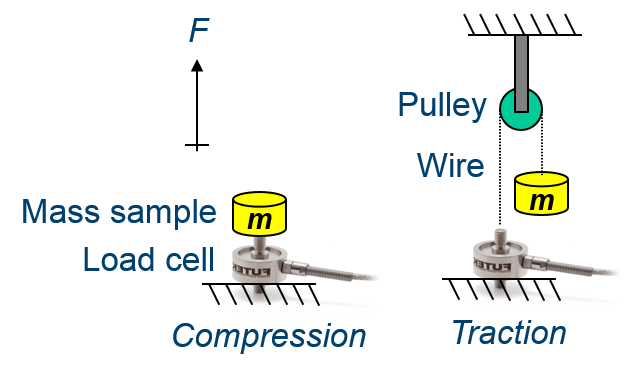
\includegraphics[width=0.7\textwidth]{Sketch.png}
                \centering
                \caption{Sketch of the Case}
                \label{fig:sketch}
        \end{figure}

        Each mass sample is applied to the load cell for a few seconds and the correspondent electrical output is recorded (the sampling frequency is \( f_s=100 \: H\!z \)). This produces a noisy signal like the one shown in Figure~.

        \begin{figure}[!ht]
                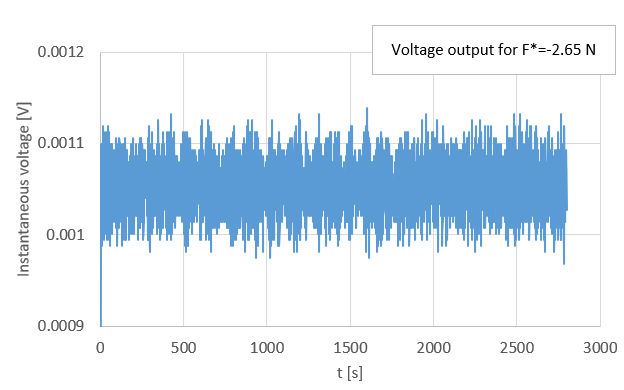
\includegraphics[width=0.7\textwidth]{Noise.png}
                \centering
                \caption{Noisy Load Cell signal example}
                \label{fig:noise}
        \end{figure}

        The voltage output histories and the corresponding values of the reference force, \( F^* \), are listed in the Table and provided in the form of MATLAB workspaces. Each workspace contains the vector of the readings in Volt (remember that the sampling frequency is \( f_s = 100 H\!z \)). In Table~\ref{tab:data}, the sign of F* is as presented in the sketch, namely, \( F^* > 0 \) when the force is directed upwards, and \( F^* < 0 \) when it is directed downwards.

        \begin{table}[!ht]
                \label{tab:data}
                \begin{tabular}{|cc|cc|}
                        \hline
                        \textbf{TestID} & \( \pmb{F^* \: \left[ N \right]} \) & \textbf{TestID} & \( \pmb{F^* \: \left[ N \right]} \) \\ \hline
                        calibr01        & 0.000               & calibr09        & -5.598              \\
                        calibr02        & -0.314              & calibr10        & -10.501             \\
                        calibr03        & -0.411              & calibr11        & 0.126               \\
                        calibr04        & -0.695              & calibr12        & 1.097               \\
                        calibr05        & -0.891              & calibr13        & 2.078               \\
                        calibr06        & -1.186              & calibr14        & 4.039               \\
                        calibr07        & -1.676              & calibr15        & 8.942               \\
                        calibr08        & -2.656              & calibr16        & 13.845              \\ \hline
                \end{tabular}
                \centering
                \caption{Reference Forces}
        \end{table}

        The main objective of the laboratory is to determine the transfer function for the load cell, and estimate the uncertainty of the instrument. For that purpose, the remainder of the report is organized as follows: Section~\ref{sec:stabilized_signal} graphically stimates the acquisition time required in order to get a stabilized measure out of an accumulating averaged voltage signal, and then provides the stabilized voltage value for each test case; Section~\ref{sec:lin_regression} performs a linear regression over the averaged voltage measure in function of the reference force; Section~\ref{sec:uncertainty} provides an approximation of the uncertainty we can expect from using the coefficients obtained in Section\ref{sec:lin_regression} to estimate the value of the measured force in function of the averaged voltage signal; finally, Section~\ref{sec:resolution} provides an approximation of the resolution of the load cell based on the measured data from the test cases.

\section{Stabilized voltage measurement} \label{sec:stabilized_signal}

\section{Linear regression} \label{sec:lin_regression}

\section{Uncertainty estimation} \label{sec:uncertainty}

\section{Resolution estimation} \label{sec:resolution}

\bibliographystyle{abbrv}
\bibliography{main}

\end{document}
